\documentclass[conference]{IEEEtran}

\usepackage{colortbl}
\input{symbols.inc}

\usepackage[T1]{fontenc}

\IEEEoverridecommandlockouts

\definecolor{taskyblue}{rgb}{0.44706, 0.56078, 0.81176}         % #728fcf
\definecolor{ta2skyblue}{rgb}{0.20392, 0.39608, 0.64314}        % #3465a4
\definecolor{ta3skyblue}{rgb}{0.12549, 0.29020, 0.52941}        % #204a87


\begin{document}

\title{Verifying Multi-threaded Software with Impact\thanks{Supported by ERC project~280053, EPSRC
project~EP/H017585/1 and the Semiconductor Research Corporation (SRC) under
task~2269.002.}}

\author{
\IEEEauthorblockN{Bj\"orn Wachter}
\IEEEauthorblockA{
Department of Computer Science\\
University of Oxford\\
Email: bjoern.wachter@cs.ox.ac.uk}
\and
\IEEEauthorblockN{Daniel Kroening}
\IEEEauthorblockA{Department of Computer Science\\
University of Oxford\\
Email: daniel.kroening@cs.ox.ac.uk}
\and
\IEEEauthorblockN{Jo\"el Ouaknine}
\IEEEauthorblockA{
Department of Computer Science\\
University of Oxford\\
Email: joel.ouaknine@cs.ox.ac.uk}
}

% LNCS-style header
% \author{Daniel Kroening \and Jo\"el Ouaknine \and Bj\"orn Wachter}
% \institute{
% University of Oxford, United Kingdom
% }

\maketitle
\begin{abstract}
Lazy abstraction with interpolants,
also known as the \emph{Impact algorithm},
is en vogue as a state-of-the-art software model-checking technique for sequential programs.
However, a direct extension of the Impact algorithm 
to concurrent programs is bound to
be inefficient as it has to explore all thread interleavings,
which leads to control-state explosion.
To this end, we present a new algorithm that combines
a new, symbolic form of partial-order reduction with Impact.
Our algorithm carries out the dependence analysis
on-the-fly while constructing the abstraction
and is thus able to deal precisely with dynamic dependencies
arising from accesses to tables or pointers
--- a setting where classical static partial-order reduction techniques struggle.
We have implemented the algorithm in a prototype
tool that analyses concurrent C program with POSIX threads 
and evaluated it on a number of benchmark programs. 
To our knowledge, this is the first application
of an Impact-like algorithm to concurrent programs.
\end{abstract}

\section{Introduction}

Concurrent software is gaining importance owing to the advent of
power-efficient multi-core architectures.  Model checking for concurrent
software is thus one of the most pressing problems facing the verification
community.  Concurrent software in C/C++ is usually written using mainstream
APIs such as POSIX, or via a combination of language and library
support as in Java.  Typically, multiple threads are spawned---either
up-front or dynamically---which communicate via shared variables.  While
software verification generally has to cope with \emph{data state
explosion}, threads introduce the problem of state explosion due to the
need of keeping track of a plethora of thread interleavings.

% lazy abstraction with interpolants for data

Lazy abstraction with interpolants~\cite{DBLP:conf/cav/McMillan06}, also known as the \emph{Impact
algorithm}, has emerged as one of the most efficient algorithms for
addressing the data state explosion problem for sequential programs.
\emph{Impact} unwinds the control-flow graph of the program in the form of
an abstract reachability tree.  Whenever the exploration arrives at an error
state, the nodes on the error path are annotated with invariants that prove
infeasibility of the error path.  The crux of the algorithm is a covering
check that allows the algorithm to soundly stop the unwinding and terminate
with a correctness proof of the program.  The underlying observation is that
tree nodes represent sets of program states which are related by subset
relations.  Roughly, a node $w$ labeled with $x>0$ ``contains'' a node $v$
labeled with $x>1$.  If we have established that the superset node $w$
cannot be on an error path, we do not need to search for an error path from
subset node $v$.  This combination of low-cost program unwindings combined
with path-based refinement and covering checks gives rise to an efficient
software model checking algorithm.

However, the original \emph{Impact} algorithm has been devised for
sequential code only.  A direct extension of \emph{Impact} to multi-threaded
programs amounts to an enumeration of thread interleavings.  Let us
illustrate this with the example program with two threads given in
Figure~\ref{figure:art:array}.  On the left-hand side of the figure, the
state graph with the complete set of interleavings is shown.  Note that
there is a diamond-shaped structure where program paths merge, e.g.,
executing instruction $A$ and then $a$ leads to the same state as executing
$a$ first and then $A$, making certain sequences of instructions redundant. 
This situation is very common in multi-threaded programs.

\begin{figure}

\begin{center}
\centering

\scriptsize

  \begin{tabular}{|l|l|l|}\hline
  
    \rowcolor{taskyblue!20}
    \texttt{main()}                        & thread $\thread_1$          & thread $\thread_2$ \\ \hline
    \texttt{assume(i!=j);}                 &                             & \\
    \texttt{v[i]=0; v[j]=0;}               & $A:$ \texttt{v[i]=1;}       & $a:$ \texttt{v[j]=-2;} \\
    \texttt{pthread\_create}($\thread_1$); & $B:$ \texttt{v[i]=v[i]+1;}  & $b:$ \texttt{v[j]=v[j]+1;}\\
    \texttt{pthread\_create}($\thread_2$); & $C:$ \texttt{v[i]=v[j]; }   & $c:$ \texttt{v[i]=v[i]+1;} \\
    \texttt{pthread\_join}($\thread_1$);   &                             & \\
    \texttt{pthread\_join}($\thread_2$);   &                             & \\
    \texttt{assert(v[j] $\geq$ 0);} & & \\\hline
  \end{tabular}
\end{center}

\begin{center}

\centering
\begin{tabular}{p{0.2\textwidth}p{0.2\textwidth}}
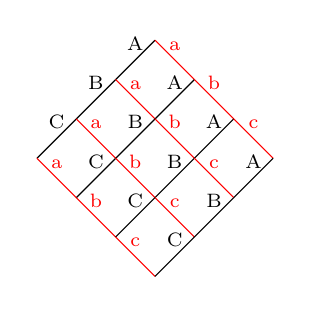
\begin{tikzpicture}[scale=0.5]
  % root
  \node (v0) at (0,6) {};
  % level 0
  \node (v1) at (-1,5) {};
  \node (v2) at (1,5) {};
  % level 1
  \node (v3) at (-2,4) {};
  \node (v4) at (0,4) {};
  \node (v5) at (2,4) {};
  % level 2
  \node (v6) at (-3,3) {};
  \node (v7) at (-1,3) {};
  \node (v8) at (1,3) {};
  \node (v9) at (3,3) {};
  % level 3
  \node (v10) at (-2,2) {};
  \node (v11) at (0,2) {};
  \node (v12) at (2,2) {};
  % level 4
  \node (v13) at (-1,1) {};
  \node (v14) at (1,1) {};
  % level 5
  \node (v15) at (0,0) {};


  % level 0
  \draw (v0.center) to node[above] {\scriptsize A} (v1.center);
  \draw[color=red] (v0.center) to node[above] {\scriptsize a} (v2.center);
  
  % level 1
  \draw (v1.center) to node[above] {\scriptsize B} (v3.center);
  \draw[color=red] (v1.center) to node[above] {\scriptsize a} (v4.center);
  \draw (v2.center) to node[above] {\scriptsize A} (v4.center);
  \draw[color=red] (v2.center) to node[above] {\scriptsize b} (v5.center);

  % level 2
  \draw (v3.center) to node[above] {\scriptsize C} (v6.center);
  \draw[color=red] (v3.center) to node[above] {\scriptsize a} (v7.center);
  \draw (v4.center) to node[above] {\scriptsize B} (v7.center);
  \draw[color=red] (v4.center) to node[above] {\scriptsize b} (v8.center);
  \draw (v5.center) to node[above] {\scriptsize A} (v8.center);
  \draw[color=red] (v5.center) to node[above] {\scriptsize c} (v9.center);

  % level 3
  \draw[color=red] (v6.center) to node[above] {\scriptsize a} (v10.center);
  \draw (v7.center) to node[above] {\scriptsize C} (v10.center);
  \draw[color=red] (v7.center) to node[above] {\scriptsize b} (v11.center);
  \draw (v8.center) to node[above] {\scriptsize B} (v11.center);
  \draw[color=red] (v8.center) to node[above] {\scriptsize c} (v12.center);
  \draw (v9.center) to node[above] {\scriptsize A} (v12.center);

  % level 4
  \draw[color=red] (v10.center) to node[above] {\scriptsize b} (v13.center);
  \draw (v11.center) to node[above] {\scriptsize C} (v13.center);
  \draw[color=red] (v11.center) to node[above] {\scriptsize c} (v14.center);
  \draw (v12.center) to node[above] {\scriptsize B} (v14.center);

  % level 5
  \draw[color=red] (v13.center) to node[above] {\scriptsize c} (v15.center);
  \draw (v14.center) to node[above] {\scriptsize C} (v15.center);
\end{tikzpicture}

&
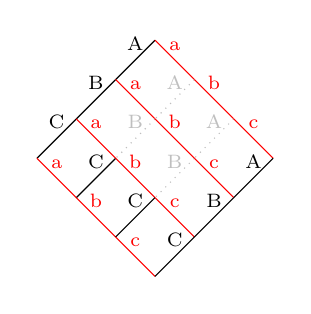
\begin{tikzpicture}[scale=0.5]
  % root
  \node (v0) at (0,6) {};
  % level 0
  \node (v1) at (-1,5) {};
  \node (v2) at (1,5) {};
  % level 1
  \node (v3) at (-2,4) {};
  \node (v4) at (0,4) {};
  \node (v5) at (2,4) {};
  % level 2
  \node (v6) at (-3,3) {};
  \node (v7) at (-1,3) {};
  \node (v8) at (1,3) {};
  \node (v9) at (3,3) {};
  % level 3
  \node (v10) at (-2,2) {};
  \node (v11) at (0,2) {};
  \node (v12) at (2,2) {};
  % level 4
  \node (v13) at (-1,1) {};
  \node (v14) at (1,1) {};
  % level 5
  \node (v15) at (0,0) {};


  % level 0
  \draw (v0.center) to node[above] {\scriptsize A} (v1.center);
  \draw[color=red] (v0.center) to node[above] {\scriptsize a} (v2.center);
  
  % level 1
  \draw (v1.center) to node[above] {\scriptsize B} (v3.center);
  \draw[color=red] (v1.center) to node[above] {\scriptsize a} (v4.center);
  \draw[dotted,lightgray] (v2.center) to node[above,color=lightgray] {\scriptsize A} (v4.center);
  \draw[color=red] (v2.center) to node[above] {\scriptsize b} (v5.center);

  % level 2
  \draw (v3.center) to node[above] {\scriptsize C} (v6.center);
  \draw[color=red] (v3.center) to node[above] {\scriptsize a} (v7.center);
  \draw[dotted,lightgray] (v4.center) to node[above,color=lightgray] {\scriptsize B} (v7.center);
  \draw[color=red] (v4.center) to node[above] {\scriptsize b} (v8.center);
  \draw[dotted,lightgray] (v5.center) to node[above,color=lightgray] {\scriptsize A} (v8.center);
  \draw[color=red] (v5.center) to node[above] {\scriptsize c} (v9.center);

  % level 3
  \draw[color=red] (v6.center) to node[above] {\scriptsize a} (v10.center);
  \draw (v7.center) to node[above] {\scriptsize C} (v10.center);
  \draw[color=red] (v7.center) to node[above] {\scriptsize b} (v11.center);
  \draw[dotted,color=lightgray] (v8.center) to node[above] {\scriptsize B} (v11.center);
  \draw[color=red] (v8.center) to node[above] {\scriptsize c} (v12.center);
  \draw (v9.center) to node[above] {\scriptsize A} (v12.center);

  % level 4
  \draw[color=red] (v10.center) to node[above] {\scriptsize b} (v13.center);
  \draw (v11.center) to node[above] {\scriptsize C} (v13.center);
  \draw[color=red] (v11.center) to node[above] {\scriptsize c} (v14.center);
  \draw (v12.center) to node[above] {\scriptsize B} (v14.center);

  % level 5
  \draw[color=red] (v13.center) to node[above] {\scriptsize c} (v15.center);
  \draw (v14.center) to node[above] {\scriptsize C} (v15.center);
\end{tikzpicture}
\end{tabular}
\end{center}
\vspace{-.75cm}
\caption{An example program (top) and its complete interleaving (left) and reduced interleaving semantics (right).
\label{figure:art:array}
\vspace{-.5cm}
}

\end{figure}

\emph{Impact} produces the full program unwinding,
as the exploration of the abstract tree has to reach an error location to
discover the right invariants.  The algorithm may find identical invariants
for redundant paths, but this does not prune the abstract exploration, as,
at that point, the program paths have already been completely unwound. 

\mph{Force cover}, an optimization of \emph{Impact}, improves this
situation by giving \emph{Impact} the power to discover that certain program
executions merge without fully exploring the paths to the error location. 
This reduces the number of paths to be explored.  On our example, the
application of force covers results in a tree of a similar size as the
graph on the left-hand side of Figure~\ref{figure:art:array}.  In
particular, even with force covers, \emph{Impact} still explores \emph{all}
thread interleavings in our example, which can be prohibitively expensive.

%
\begin{wrapfigure}[10]{r}{0.4\linewidth}
\centering
\vspace{-0.75cm}
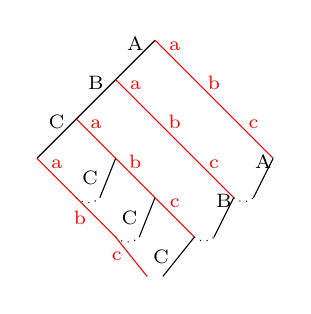
\begin{tikzpicture}[scale=0.5]
  % root
  \node (v0) at (0,6) {};
  % level 0
  \node (v1) at (-1,5) {};
  \node (v2) at (1,5) {};
  % level 1
  \node (v3) at (-2,4) {};
  \node (v4) at (0,4) {};
  \node (v5) at (2,4) {};
  % level 2
  \node (v6) at (-3,3) {};
  \node (v7) at (-1,3) {};
  \node (v8) at (1,3) {};
  \node (v9) at (3,3) {};
  % level 3
  \node (v10) at (-2,2) {};
  
  \node (v10p) at (-1.4,2) {};
  
  \node (v11) at (0,2) {};
  \node (v12p) at (2.5,2) {};

   \node (v12) at (2,2) {};

  % level 4
  \node (v13) at (-1,1) {};
  
  \node(v13p) at (-.4,1) {};
  
  \node (v14) at (1,1) {};
  \node (v14p) at (1.5,1) {};

  % level 5
  \node (v15) at (-.2,0) {};
  \node (v15p) at (.2,0) {};

  % level 0
  \draw (v0.center) to node[above] {\scriptsize A} (v1.center);
  \draw[color=red] (v0.center) to node[above] {\scriptsize a} (v2.center);
  
  % level 1
  \draw (v1.center) to node[above] {\scriptsize B} (v3.center);
  \draw[color=red] (v1.center) to node[above] {\scriptsize a} (v4.center);
  %\draw[dotted,lightgray] (v2.center) to node[above,color=lightgray] {\scriptsize A} (v4.center);
  \draw[color=red] (v2.center) to node[above] {\scriptsize b} (v5.center);

  % level 2
  \draw (v3.center) to node[above] {\scriptsize C} (v6.center);
  \draw[color=red] (v3.center) to node[above] {\scriptsize a} (v7.center);
  %\draw[dotted,lightgray] (v4.center) to node[above,color=lightgray] {\scriptsize B} (v7.center);
  \draw[color=red] (v4.center) to node[above] {\scriptsize b} (v8.center);
  %\draw[dotted,lightgray] (v5.center) to node[above,color=lightgray] {\scriptsize A} (v8.center);
  \draw[color=red] (v5.center) to node[above] {\scriptsize c} (v9.center);

  % level 3
  \draw[color=red] (v6.center) to node[above] {\scriptsize a} (v10.center);
  \draw (v7.center) to node[left] {\scriptsize C} (v10p.center);

  \draw[dotted](v10.center) to [out=-45,in=225] node {} (v10p.center) {};
  
  \draw[color=red] (v7.center) to node[above] {\scriptsize b} (v11.center);
  %\draw[dotted,color=lightgray] (v8.center) to node[above] {\scriptsize B} (v11.center);
  \draw[color=red] (v8.center) to node[above] {\scriptsize c} (v12.center);
  \draw (v9.center) to node[above] {\scriptsize A} (v12p.center);
  
  \draw[dotted](v12.center) to [out=-45,in=225] node {} (v12p.center) {};

  % level 4
  \draw[color=red] (v10.center) to node[left] {\scriptsize b} (v13.center);
  \draw (v11.center) to node[left] {\scriptsize C} (v13p.center);
  
  \draw[dotted](v13.center) to [out=-45,in=225] node {} (v13p.center) {};
  
  \draw[color=red] (v11.center) to node[above] {\scriptsize c} (v14.center);
  

  \draw (v12.center) to node[above] {\scriptsize B} (v14p.center);

  \draw[dotted](v14.center) to [out=-45,in=225] node {} (v14p.center) {};

  % level 5
  \draw[color=red] (v13.center) to node[left] {\scriptsize c} (v15.center);
  \draw (v14.center) to node[left] {\scriptsize C} (v15p.center);
\end{tikzpicture}
\caption{\emph{Impact} with POR and force cover
\label{fig:portree} }
\end{wrapfigure}
%
A principal method to reduce the number of interleavings in the exploration
of concurrent programs is \emph{partial-order reduction} (POR)~\mbox{\cite{DBLP:books/sp/Godefroid96,DBLP:conf/cav/Peled93,DBLP:conf/apn/Valmari89,DBLP:journals/fmsd/Godefroid05}}. 
The right-hand side of Figure~\ref{figure:art:array} shows an exploration reduced by means
of partial-order reduction.  A key contribution of this paper is a novel
combination of \emph{Impact} with POR, which produces
the abstract tree shown in Figure~\ref{fig:portree}. 
\emph{Impact} with force cover alone explores a tree with five further nodes, as it does not
know in advance that the executions merge, while partial-order reduction is
able to discover this earlier. Discovering redundant paths early on during the
exploration is crucial to avoid path explosion.


\paragraph*{Contributions}

\begin{itemize}
  \item We present an extension of the Impact algorithm to concurrent software.
  \item We show how to combine partial-order reduction with Impact.
        Due to a subtle interplay between node coverings and POR,
        obtaining a sound verification procedure is non-trivial.
        To this end, we give a general framework to prove such combinations correct,
        and an algorithm based on this framework which combines
        Impact with monotonic partial-order reduction~\cite{DBLP:conf/tacas/WangYKG08}.
  \item We compare the effect of partial-order reduction
        and force covers; our conjecture is that the two techniques yield
        orthogonal benefits and are best combined.
\end{itemize}

We present background and basic definitions in Section~\ref{sec:basic}. 
We develop a variant of the \emph{Impact} algorithm for concurrent software
in Section~\ref{sec:algo}.  We present a combination of partial-order
reduction and \emph{Impact} in Section~\ref{sec:partial}.  Experimental
results are discussed in Section~\ref{sec:experiments}.

\section{Basic Definitions}
\label{sec:basic}

\paragraph*{Program semantics}

We consider a concurrent program $\program$ composed of a finite set of
threads \threads, which communicate by performing operations on
shared variables.

A state of a concurrent system consists of the local states $\lstates$ of
each thread, i.e., the value of the thread's program counter given by a
program location $l \in \locs$ and values of the local variables of the
thread, and of the shared states $\sstates$, i.e., values for communication
objects such as locks, tables and the like.  Thus, we have a global state
space $\states=\sstates\times\lstates$.

A global control location is a function $\locvec:\threads \to \locs$ from
threads to control locations.  Let $\locvecs$ be the set of global control
locations.  The global location in state $s$ is denoted by $\locvec(s)$. 
For a given global location $\locvec$ and thread $\thread$, we write
$\locvec_\thread$ as a shorthand for $\locvec(\thread)$.  By
$\locvec[\thread\mapsto l]$, we denote the global location where the
location of thread $\thread$ maps to $l$, while the locations for 
all other threads $\thread'$ remain unchanged.

We characterize program data in terms of formulas in standard first-order
logic.  We denote the set of well-formed formulas over symbols $\Sigma$ by
$\wff(\Sigma)$.  For a given formula $F$ we denote the set of formulas over
the same symbols by $\wff(F)$.  

%Let $\vars=\svars \cup \lvars$ be the
%vocabulary that represents the program variables, which consist of the
%shared variables $\svars$ and local variables $\lvars$ respectively.  
Let $\vars$ be the vocabulary that represents the program variables.
A state formula is a formula in $\wff(V)$ and represents a set of global states.  
A transition formula, from now on, typically denoted by the letter
$R$, is a formula in $\wff(V\cup V')$.

Formally, we model a program  as a pair $(\init,\threads)$ where $\init \in
\wff(V)$ is the initial-state predicate, and $\threads$ a finite set of
threads.  We assume that the set of threads is endowed with some total order
$<$.  A thread $\thread \in \threads$ is a tuple
$\thread=(\locs,\locinit,\locfinal,\actions)$ consisting of a finite set of
control locations $\locs$, an initial location $\locinit \in \locs$, an
error location $\locfinal$, and a set of actions $\actions$.  An action is a
pair $a=(l,N) \in \locs \times 2^{\wff(\vars \cup \vars') \times \locs}$,
consisting of a current location $l$ and a set of successor control
locations $l'$, each associated with a transition constraint. 
An assignment \mbox{\texttt{$l_1$: x=y+1; $l_2$: $\ldots$}} 
is represented as \mbox{$(l_1,\{(x'=y+1\wedge y'=y;l_2)\})$}.
An assertion \mbox{\texttt{$l_1$: assert(x<y); $l_2$: $\ldots$}} becomes an action
$(l_1,\{(x\geq y\wedge x'=x \wedge y'=y,\locfinal),(x<y\wedge x'=x \wedge y'=y,l_2)\})$,
which enters the error location $\locfinal$ if the condition is violated.
Sets of successors are used to represent branching control flow, e.g., the encoding
of the \texttt{if}-statement
\mbox{
$
\texttt{$l_1$: if(x==1) goto $l_3$; $l_2$: $\ldots$}
$
}
is \mbox{$(l_1,\{(x=1\wedge x'=x,l_3),(x\neq1\wedge x'=x,l_2)\})$}. 


We write $\locs(\thread)$ and $\actions(\thread)$ to
denote the locations and actions of a thread.  For an action $a=(l,N)\in
\actions(\thread)$ of thread $\thread$, action $a$ is enabled at location
$l$ and at global location $\locvec$ if $a$ is enabled at $\locvec_\thread$. 
We assume that exactly one action $a_{\thread,l}$ of any given $\thread$ is
enabled at any location $l\in\locs$.

The control-flow graph $CFG_\thread=(\locinit,E)$ of thread
$\thread=(\locs,\locinit,\locfinal,\actions)$ is defined by entry node
$\locinit$ and edges $E=\bigcup_{a\in\actions(\thread)} E_a$ where
$E_a=\{(l,l')\in \locs\times\locs \mid a=(l,N), (R,l')\in N\}$.  The
control-flow nodes are topologically ordered.  We say that an action $a$
induces a back edge if $E_a$ contains a back edge.

We say that an action $a=(l,N) \in \thread $ is enabled at a state if
$a$ is enabled at global location $\locvec(s)$.
We denote the enabled actions at a state $s$ by $\mathit{enabled}(s)$.
We assume that an action $a=(l,N)$ defines a total function
$
\{s \in \states \mid a \in \mathit{enabled}(s)\} \to \states
$
on all program states for which it is enabled.

For ease of notation, we identify $a$ with this function
and write $a(s)$ to denote the successor of a state $s$ under action $a$.

\paragraph*{Invariants and Correctness Proofs}

A program path $\pi$ is a sequence $\pathsequence$.
For a thread~$\thread$, and $l,l'\in \locs(\thread)$ with $l\neq l'$,
we write $l \sqsubset l'$ if there exists a program path
from $l$ to $l'$.

A path is an \emph{error path} if $\locvec_0$ is the vector of initial
locations for all threads, and $\locvec_{N-1}$ contains an error location of
a thread.  We denote by $\formula(\pi)$ the sequence of formulas
$\init^{(0)} \wedge R_0^{(0)}, \ldots R_{N-1}^{(N-1)}$ obtained by shifting
each $R_i$ $i$ time frames into the future.  We say that $\pi$ is feasible
if $\bigwedge R_i^{(i)}$ is logically satisfiable.  A solution to $\bigwedge
R_i^{(i)}$ corresponds to a program execution assigning values to the
program variables at each execution step.  The program is said to be safe if
all error paths are infeasible.

An \emph{inductive invariant} is a mapping $I:  \locvecs \to \wff(V)$ such that
%
$\init \Rightarrow I(\locvecinit)$
and for all locations $\locvec \in \locvecs$, all threads $\thread\in\threads$,
and actions $a=(l,R,l')\in \thread$ in thread $\thread$ enabled in $\locvec$,
we have $I(\locvec)\wedge R \Rightarrow I(\locvec[\thread\mapsto l'])$.
A \emph{safety invariant} is an inductive invariant with
$I(\locvec)\equiv \mathit{False}$ for all error locations $\locvec$.
If there is a safety invariant the program is safe.

\paragraph*{Interpolants}

In case a path is infeasible, an explanation can be extracted in the form of
an interpolant.   To this end, we define \emph{sequent
interpolants}~\cite{DBLP:journals/tcs/McMillan05}.  A sequent interpolant
for formulas $A_1,\ldots,A_N$, is a sequence $\widehat A_1,\ldots, \widehat
A_N$ where the first formula is equivalent to true $\widehat A_1\equiv
\mathit{True}$, the last formula is equivalent to false $\widehat A_N\equiv
\mathit{False}$, consecutive formulas imply each other, i.e., for all
$i\in\{1,\ldots,N\}$, $\widehat A_{i-1}\wedge A_i \Rightarrow \widehat A_i$,
and, the $i$-th sequent is a formula over the common symbols of its prefix
and postfix, i.e., for all $i\in\{1,\ldots N\}$, $\widehat A_{i}\in
\wff(A_1,\ldots,A_i) \cap \wff(A_{i+1},\ldots,A_N)$.  For certain
theories, quantifier-free interpolants can be generated for inconsistent,
quantifier-free sequences
$A_1,\ldots,A_N$~\cite{DBLP:journals/tcs/McMillan05}.

\section{Impact Algorithm for Concurrent Programs}
\label{sec:algo}

We now present an extension of the original Impact algorithm to
concurrent programs.  The algorithm returns either a safety invariant for a
given program, finds a counterexample or diverges (the verification problem
is undecidable).  To this end, the algorithm constructs an abstraction of
the program in the form of an abstract reachability tree, which corresponds
to a program unwinding annotated with invariants.

\begin{center}
  \begin{define}[ART]
    An \emph{abstract reachability tree} (ART) $\art$ for program $\program$ is a tuple
    $(V,\epsilon,\transby{},\covers)$ consisting of a tree with nodes $V$, root node
    $\epsilon \in V$, edges $\transby{} \subseteq V^2$, and a covering relation $\covers
    \subseteq V^2$ between tree nodes such that:
    %
    \begin{itemize}
      \item every nodes $v\in V$ is labeled with a tuple $(\locvec,\annotation)$ consisting of
      a current global control location $\locvec$, and a state formula
      $\annotation$.
      We write $\locvec(v)$ and $\annotation(v)$ 
      to denote the control location and annotation, respectively, of node $v$.

      \item edges correspond to program actions, and
      tree branching represents both branching in the control flow
      within a thread and thread interleaving.  Formally, an edge is a
      tuple $(v,\thread,R,w)$ where $v,w \in V$,
      $\thread\in\threads$, and $R$ the transition
      constraint of the corresponding action.
    \end{itemize} 
    %
    We write $v\transby{\thread, R} w$ if there exists an edge $(v,\thread,R,w)\in
    \transby{}$.  We denote by $\transbystar{}$ the transitive closure of
    $\transby{}$.
  \end{define}         
\end{center}

To put abstract reachability trees to work for proving program correctness
for unbounded executions, we need a criterion to prune the tree 
without missing any error paths.
This role is assumed by the covering relation $\covers$.

Intuitively, the purpose of node labels is to represent inductive invariants, i.e.,
over-approximations of sets of states, and the covering relation is the
equivalent of a subset relation between nodes.  Suppose that two nodes $v,w$
share the same control location, and $\annotation(v)$ implies
$\annotation(w)$.  If there was a feasible error path from~$v$, there would
be a feasible error path from~$w$.  Therefore, if we can find a safety
invariant for $w$, we do not need to explore successors of $v$, as
$\annotation(v)$ is at least as strong as the already sufficient invariant $\annotation(w)$.

Note that, therefore, if $w$ is safe, all nodes in the subtree rooted
in $v$ are safe as well.  Therefore, a node is covered if and only if the
node itself or any of its ancestors has a label implied by another node's
label at the same control location.

To obtain a proof from an ART, the ART needs to fulfill
certain conditions, summarized
in the following definition:

\begin{center}
  \begin{define}[Safe ART]
    Let $\art=(V,\epsilon,\transby{},\covers)$ be an ART.
    \begin{itemize}
    \item $\art$ is \emph{well-labeled} if the labeling is
          inductive, i.e., 
          $\forall (v,\thread,R,w) \in \transby {}:\ \locvec(v) = \locvec(w) \wedge \annotation(v) \wedge R 
           \Rightarrow \annotation(w)'$
          and compatible with covering, i.e., 
          $(v,w)\in\covers:\ \annotation(v)\Rightarrow \annotation(w)$ and
          $w$ not covered.
    \item $\art$ is \emph{complete} if all of its nodes are covered,
    or have an out-going edge for every action that is enabled at $\locvec$.
    \item $\art$ is \emph{safe} if all error nodes are labeled with
    $\mathit{False}$.
    \end{itemize}
  \end{define}
\end{center}

\begin{theorem}
  If there is a safe, complete, well-labeled ART of program $\program$, the program is safe.
\end{theorem}
\begin{proof} 
  As in \cite{DBLP:conf/cav/McMillan06},
  the labeling immediately gives a safety invariant $M$,
  $M(\locvec') = \bigvee \{ \annotation(v) \mid \locvec(v) = \locvec'\}$. 
  \qed
\end{proof}

\vspace{-.25cm}

\begin{algorithm*}
\vspace{-.25cm}
\begin{tabular}{p{0.3\textwidth}p{0.3\textwidth}p{0.3\textwidth}}
\begin{algorithmic}[1]
\footnotesize

\Procedure {main}{$ $}
	\State $Q := \{ \epsilon \}$, $\covers := \emptyset$
	\While { $Q \neq \emptyset$}
		\State select and remove $v$ from $Q$
		\State $\prog{Close}(v)$
		\If {$v$ not covered}
			\If { $error(v)$ }
	 			\State $\prog{Refine}(v)$
			\EndIf
  		\State $\prog{Expand}(v)$
		\EndIf
	\EndWhile
	\State
	\Return $\program$ is safe
\EndProcedure  \\
\Procedure {expand}{$v$}
    \For { $ \thread \in \threads$}
		\State $\prog{Expand-thread}(\thread,v)$
    \EndFor
\EndProcedure 
\end{algorithmic}
&
\begin{algorithmic}[1]
\footnotesize

\makeatletter\setcounter{ALG@line}{14}\makeatother

\Procedure {expand-thread}{$\thread, v$}
  
    \State $(\locvec,\annotation) := v$
    	\For { $(l,N) \in \actions(\thread)$ with $\locvec_\thread=l$}
		\For { $(R,l') \in N$}
		\State $w:=$ fresh node 
    		\State $\locvec(w):=\locvec[\thread\mapsto l']$
      		\State $\annotation(w) := \mathit{True}$
      		\State $Q := Q \cup \{w\}$, $V := V \cup \{w\}$
      		\State $\transby {} := \transby {} \cup \{ (v,\thread,R,w) \}$   \label{algo:impact:expand:trans}
		\EndFor
   	\EndFor
\EndProcedure 
\\
\Procedure {close}{$v$}
  \For {$w \in V^{\prec v}:$ $w$ uncovered}
         \If {$\locvec(v)=\locvec(w) \wedge \annotation(v) \Rightarrow \annotation(w)$}
        		\State $\covers := \covers \cup \{ (v,w) \}$
         		\State $\covers := \covers \setminus \{(x,y)\in \covers \mid v \transbystar{} y \}$
         \EndIf	
  \EndFor
\EndProcedure


\end{algorithmic}
&
\begin{algorithmic}[1]
\footnotesize

\makeatletter\setcounter{ALG@line}{29}\makeatother

\Procedure {refine}{$v$}
  \If  {$v$ not error node or $\annotation(v) \equiv \mathit{False}$}
    \State \Return
  \EndIf 
	\State $\pi :=v_0,\ldots v_N $  path from $\start$ to $v$
	\If {$\formula(\pi)$ has interpolant $A_0 \ldots A_N$ }
			\For { $ i = 0 \ldots N$}
				\State $\annotation := A_i^{-i}$
				\If {$\annotation(v_i) \not \vDash \annotation$}
					\State $Q := Q \cup \{ w \mid w \covers v_i \}$
					\State $\covers := \covers \setminus \{ (w,v_i) \mid w \covers v_i \}$
					\State $\annotation(v_i) := \annotation(v_i) \wedge \annotation$
				\EndIf
			\EndFor
      \For { $w \in V$ s.t. $w \transbystar{} v$}
      	\State $\prog{Close}(w)$
      \EndFor
	\Else
		\State \ abort (program unsafe)
	\EndIf

\EndProcedure 

\end{algorithmic}
\end{tabular}
\vspace{-.5cm}
\caption{Impact with support for concurrent programs\label{algo:impact}}
\end{algorithm*}

\subsection{Concurrent Impact with Full Interleaving}
The concurrent version of the \impact algorithm we describe next
(Algorithm~\ref{algo:impact}) constructs an ART by alternating 
three different operation on nodes: \prog{Expand}, \prog{Refine}, and \prog{Close}.
At all times, the algorithm maintains the invariant that the tree is well-labeled and safe,
i.e., to produce a correctness proof the algorithm needs to make the tree complete.

To keep track of nodes where the tree is incomplete,
uncovered leaf nodes are kept in a work list $Q$.

\prog{Expand} takes an uncovered leaf node and computes its successors.
     To this end, it iterates over all threads.  For every enabled action,
     it creates a fresh tree node $w$, and sets its location to the control
     successor $l'$ given by the action.  To ensure that the labeling is
     inductive, the formula $\annotation(w)$ is set to $\mathit{True}$.  Then
     the new node is added to the work list $Q$.  Finally, a tree edge is
     added (Line~\ref{algo:impact:expand:trans}), which records the step from
     $v$ to $w$ and the transition formula $R$.  Note that if $w$ is an
     error location, the labeling is not safe; in which case, we need to
     refine the labeling, invoking operation \prog{Refine}.
          
\prog{Refine} takes an error node $v$ and, detects if the error path is feasible
     and, if not, restores a safe tree labeling.  First, it determines if
     the unique path $\pi$ from the initial node to $v$ is feasible by
     checking satisfiability of $\formula(\pi)$.  If $\formula(\pi)$ is
     satisfiable, the solution gives a counterexample in the form of a
     concrete error trace, showing that the program is unsafe. Otherwise, an
     interpolant is obtained, which is used to refine the labeling.  Note
     that strengthening the labeling may destroy the well-labeledness of the
     ART.  To recover it, pairs $w \covers v_i$ for strengthened nodes $v_i$
     are deleted from the relation, and the node $w$ is put into the work
     list again.

\prog{Close} takes a node $v$ and checks if $v$ can be added to the covering
     relation.  As potential candidates for pairs $v \covers w$, it only
     considers nodes created before $v$, denoted by the set $V^{\prec
     v}\subsetneq V$.  This is to ensure stable behavior, as covering in
     arbitrary order may uncover other nodes, which may not terminate.  Thus
     only for uncovered nodes $w \in V^{\prec v}$, it is checked if
     $\locvec(w)=\locvec(v)$ and $\annotation(v)$ implies $\annotation(w)$. 
     If so, $(v,w)$ is added to the covering relation $\covers$.  To restore
     well-labeling, all pairs $(x,y)$ where $y$ is a descendant of $v$,
     denoted by $v\transbystar{} y$, are removed from $\covers$, as $v$ and
     all its descendants are covered.

\prog{Main} first initializes the queue with the initial node~$\epsilon$,
     and the relation $\covers$ with the empty set.  It then runs the main
     loop of the algorithm until $Q$ is empty, i.e., until the ART is
     complete, unless an error is found which exits the loop.  In the main
     loop, a node is selected from $Q$.  First, \prog{Close} is called to try
     and cover it.  If the node is not covered and it is an error node,
     \prog{Refine} is called.  Finally, the node is expanded, unless it was
     covered, and evicted from the work list.
           
An important optimization of the algorithm is another subroutine, called
\emph{force cover}.  Initially, all new nodes are labeled with invariant
$\mathit{True}$.  Therefore, they will not be covered by an existing node
with a non-trivial invariant, although this may be a permissible labeling. 
To check coverage, force cover finds the nearest common ancestor of two
nodes and then checks the characteristic formula to the new node to see if
the invariant of the other node also holds at the new node.  
Beyer~\cite{DBLP:conf/fmcad/BeyerW12}
showed that this optimization is essential for the performance of \emph{Impact}.

Wrapping up the extension of the original Impact algorithm to concurrent
programs: the single control location becomes a vector, and the
\prog{expand} routine enumerates all possible interleavings.  
This algorithm is very inefficient in its basic form: due to the full interleaving
semantics, the number of global control locations grows very quickly.  
We shall amend this in the next section.


\section{Partial Order Reduction}
\label{sec:partial}

Performing a thread interleaving at every step would be prohibitively expensive.
\emph{Impact} needs some way of reducing interleaving.
Therefore, we present an algorithm that combines partial-order reduction with
the \emph{Impact} algorithm.  
A very simple kind of partial order reduction is to only allow interleaving
when shared-variable accesses occur, however a much stronger reduction is possible
in many cases.
In this section, we consider a more advanced partial exploration strategy
that generates monotonic program paths $\Pi_{\mathit{mono}}$, wherein consecutive independent
actions only occur in the order of increasing thread ids~\cite{DBLP:conf/tacas/WangYKG08}.

Recall that  the soundness proof of the original \prog{Impact} algorithm 
rests on three pillars, namely: completeness, safety and well-labeledness of ARTs.
However, partial order reduction clashes
with the original completeness criterion of \prog{Impact} that requires the very thing we aim to avoid:
full expansion of all thread interleavings.
%Further, partial-order reduction avoids exploration of certain redundant global states
%and thus produces different invariants than a full interleaving semantics.
Thus we need a new soundness proof and, in particular, a weaker completeness criterion, to combine abstraction with
partial-order reduction.  

To this end, we introduce the new concept of \mbox{\emph{$\Pi$-completeness}}, 
which is parameterized with an exploration strategy via a set of
program paths $\Pi$, and gives a systematic framework to combine
abstraction with partial-order reduction. 
Based on this concept, we also present the dPOR-\prog{Impact} algorithm, which
explores monotonic paths and produces $\Pi_{\mathit{mono}}$-complete ARTs.

Before we come to $\Pi$-completeness and dPOR-\prog{Impact},
we first need to review some basic POR concepts and notation.

\subsection{Independence and Mazurkiewicz Equivalence}

Partial-order reduction is based on the notion of independence of actions. 
Intuitively, two actions are independent if they commute and we can execute
them in any order:
%
\begin{center}
  \begin{define}[Independence]
    Two actions $a_1$ and $a_2$ are \emph{independent}, denoted by
    $\independent{a_1}{a_2}$, if for all states $s \in \states$ where $a_1$ and
    $a_2$ are co-enabled, i.e., $a_1, a_2\in \mathit{enabled}(\locvec(s))$, we have
    \mbox{$a_1(a_2(s)) = a_2(a_1(s)))$}.  Otherwise, we say that they are
    dependent and write $\dependent{a_1}{a_2}$.
  \end{define}
\end{center}
%
Partial-order reduction techniques are based on finding a representative
subset of the interleavings avoiding the exploration of all equivalent interleavings,
i.e., interleavings that lead to equivalent orderings of actions.
This leads to the notion of Mazurkiewicz equivalence~\cite{DBLP:conf/ac/Mazurkiewicz86}:
%
\begin{center}
  \begin{define}[Mazurkiewicz equivalence]
  Two program paths are \emph{Mazurkiewicz equivalent} if they result
  from exchanging the order of two independent actions.

  We call a set of program paths $\Pi$ \emph{representative} if it contains
  a representative path for every Mazurkiewicz equivalence class. 
  \end{define}

\end{center}

An example for a representative set of program paths
are the monotonic program paths, which are defined as follows:

\begin{center}
  \begin{define}[Monotonic paths]
  A program path $\pi = \pathsequence$ is \emph{monotonic} if
  for all $i,j\in\{0,\ldots,N-1\}$ with $i<j$,
  $\independent{a_i}{a_j}$ and  $\thread_i > \thread_j$,
  we have  $j\neq i+1$.
  Let $\Pi_{mono}$ be the set of monotonic program paths.
  \end{define}
\end{center}

\subsection{\texorpdfstring{$\Pi$-completeness}{Pi-completeness}}

\begin{figure}
\centering
\begin{tikzpicture}[scale=0.8]

  \node[draw=gray!50,fill=gray!30,shape=rectangle,rounded corners,inner sep=24pt,label={[label distance=-12pt]below:{$v_2$}}] (v2) at (4,1) {};

  \node[draw=gray!70,fill=gray!10,shape=rectangle,rounded corners,inner sep=8pt] (v0) at (0,1) {$v_0$};
  \node[draw=gray!70,fill=gray!10,shape=rectangle,rounded corners,inner sep=8pt] (v1) at (2,1) {$v_1$};
  \node[draw=gray!70,fill=gray!10,shape=rectangle,rounded corners,inner sep=8pt, drop shadow={ashadow, color=red!60!black}] (u2) at (4,1) {$u_2$};
  \node[draw=gray!70,fill=gray!30,shape=rectangle,rounded corners,inner sep=8pt] (v3) at (6.5,1) {$v_3$};
  \node[draw=gray!70,fill=gray!30,shape=rectangle,rounded corners,inner sep=8pt] (v4) at (8.5,1) {$v_4$};


  \node[draw,fill,shape=circle,inner sep=1pt,label=above:{$\locvec_0$}] (s0) at (0,1.3) {};
  \node[draw,fill,shape=circle,inner sep=1pt,label=above:{$\locvec_1$}] (s1) at (2,1.3) {};
  \node[draw,fill,shape=circle,inner sep=1pt,label=above:{$\locvec_2$}] (s2) at (4,1.3) {};
  \node[draw,fill,shape=circle,inner sep=1pt,label=above:{$\locvec_3$}] (s3) at (6.5,1.3) {};
  \node[draw,fill,shape=circle,inner sep=1pt,label=above:{$\locvec_4$}] (s4) at (8.5,1.3) {};

  \draw[trans] (s0) to[out=10,in=170] node {} (s1);
  \draw[trans] (s1) to[out=10,in=170] node {} (s2);
  \draw[trans] (s2) to[out=10,in=170] node {} (s3);
  \draw[trans] (s3) to[out=10,in=170] node {} (s4);
  
  \draw[trans, very thick, draw=darkgray] (v0) -- (v1); 
  \draw[trans, very thick, draw=darkgray] (v1) -- (u2); 
  \draw[trans, very thick, draw=darkgray] (v2) -- (v3);
  \draw[trans, very thick, draw=darkgray] (v3) -- (v4);

\end{tikzpicture}
\caption{Path correspondence.
Rounded rectangles represent ART nodes $v_0,\ldots,v_4$ and $u_2$.
We have $u_2 \covers v_2$.
The gray arrows depict ART edges. 
The path $l_0 \ldots l_5$ is a control flow path.
\label{fig:example:completeness}
}
\vspace{-0.5cm}
\end{figure}

We will say that an ART $\art$ is \emph{$\Pi$-complete} with respect to a
set of program paths $\Pi$ if each path $\pi\in\Pi$ is covered by $\art$. 
Intuitively, a program path is covered if there exists a corresponding
sequence of nodes in the tree, where corresponding means that it visits the
same control locations and takes the same actions.  
In absence of covers, the matching between control paths
and sequences of nodes is straightforward.

However, a path of the ART may end in a covered node.
For example, consider the path $\locvec_0 \ldots \locvec_5$ in Figure~\ref{fig:example:completeness}.
While prefix $\locvec_0 \locvec_1 \locvec_2$ can be matched by node sequence $v_0 v_1 u_2$,
node $u_2$ is covered by node $v_2$, formally $u_2 \covers v_2$.
But how we can match the remainder of the path?
We are stuck at node $u_2$, a leaf with no out-going edges.
Our solution is to allow the 
corresponding sequence to ``climb up'' the covering order 
$\covers$ to a more abstract node, here we climb from $u_2$ to $v_2$.
Node $v_2$ in turn must have a corresponding out-going edge,
as it cannot be covered and its control location is also $\locvec_2$.
Finally, the corresponding node sequence for $\locvec_0 \ldots \locvec_4$ is $v_0 \ldots v_4$.

Figure~\ref{fig:proof:completeness} illustrates the formalization of
our notion of path correspondence.
On top of the figure, we depict a fragment of a program path with locations $l_i, l_{i+1}$ and $l_{i+2}$,
and, at the bottom, the corresponding path which climbs from node
$u_{i+1}$ to node $v_{i+1}$ where $u_{i+1}$ and $v_{i+1}$ are both
at location \mbox{$\locvec(u_{i+1}) = \locvec(v_{i+1})=\locvec_{i+1}$}
and $u_{i+1} \covers v_{i+1}$.
A corresponding path is allowed to climb up not only at one position
$i$ but at any position $i$ (or none) and at arbitrarily many positions.

This notion is formalized in the following definition:
%
\begin{center}
\begin{define}[Corresponding paths \& path cover]
  \label{def:pathcover}
  Consider a program $\program$.  Let $\art$ be an ART for $\program$ and let
  $\pi=\pathsequence$ be a program path.  A \emph{corresponding path} for
  $\pi$ in $\art$ is a sequence $v_0,\ldots,v_n$ in $\art$ such that, for all
  $i\in\{0,\ldots,N-1\}$, $\locvec(v_i) = \locvec_i$, and
  %
  \begin{align*}
    \exists u_{i+1} \in V:\ v_i \transby{\thread_i, a_i} u_{i+1} \wedge (u_{i+1}=v_{i+1} \vee u_{i+1} \covers v_{i+1})
  \end{align*}
  A program path $\pi$ is covered by $\art$ if there exists a corresponding path $v_0,\ldots,v_n$ in $\art$.
\end{define}
\end{center}


\begin{figure}
\centering
\begin{tikzpicture}[scale=0.8]

  \node (li) at (-1,.9) {$\locvec_i$};
  \node (liplus1) at (3,.9) {$\locvec_{i+1}$};
  \node (liplus2) at (7,.9) {$\locvec_{i+2}$};

  \node[draw=gray!70,fill=gray!10,shape=rectangle,rounded corners] (vi) at (-1,0) {$v_i$};
  \node[draw=gray!70,fill=gray!10,shape=rectangle,rounded corners, drop shadow={ashadow, color=red!60!black}] (uiplus1) at (2,0) {$u_{i+1}$};
  \node[draw=gray!70,fill=gray!30,shape=rectangle,rounded corners] (viplus1) at (4,0) {$v_{i+1}$};
  \node[draw=gray!70,fill=gray!30,shape=rectangle,rounded corners] (viplus2) at (7,0) {$v_{i+2}$};
  
  \draw[trans, very thick, draw=darkgray]  (vi) to node[above] {$\thread_i, a_i$} (uiplus1);
  \draw[trans, very thick, draw=darkgray]  (viplus1) to node[above] {$\thread_{i+1}, a_{i+1}$} (viplus2);
  \draw[dashed] (uiplus1) to[out=-45,in=225] node[above] {$\covers$} (viplus1);

  \draw[trans] (li) to[out=10,in=170] node[above] {$\thread_i, a_i$} (liplus1);
  \draw[trans] (liplus1) to[out=10,in=170] node[above] {$\thread_{i+1}, a_{i+1}$} (liplus2); 
\end{tikzpicture}
\caption{Illustration of Definition~\ref{def:pathcover}.
The diagram shows a fragment of an ART $\art$
with notation for the nodes of the definition.
The dashed line represents a covering edge.
\label{fig:proof:completeness}
}
\vspace{-0.5cm}
\end{figure}
%


We are now ready to define our new completeness criterion:

\begin{center}
\begin{define}[$\Pi$-completeness]
  Let $\program$ be a program and $\Pi$ a set of program paths.
  ART $\art$ for $\program $ is $\Pi$-complete if
  every path $\pi \in \Pi$ is covered by $\art$.
\end{define}
\end{center}

A $\Pi$-complete, safe, well-labeled ART constitutes
a proof of program correctness, as stated in the following proposition:

\begin{center}
\begin{proposition}
  Let $\program$ be a program.
  Let $\Pi$ be a representative set of program paths.
  Assume that $\art$ is safe, well-labeled and
  $\Pi$-complete. Then program $\program$ is safe.
  \label{proposition:picompleteness}
\end{proposition}
\end{center}

\subsection{Abstraction Algorithm}
\label{sec:abstr_alg}
%
We now combine POR with \prog{Impact}.
The obvious starting point is to modify
the \prog{Expand} function in Algorithm~\ref{algo:impact}.
We first introduce the modified expansion function
\prog{\dporexpand}. However, changing only the expansion
function turns out to be insufficient.
Due to a subtle interplay between coverings and POR,
the resulting algorithm does not guarantee $\Pi_{mono}$-completeness,
and is unsound, which we illustrate with a small example.
We then describe a method to fix this problem
and present Algorithm~\ref{algorithm:partial_order},
a sound variant of Impact with POR.

First, we change $\prog{Expand}$ such that only
monotonic paths are unwound.
To this end, instead of expanding all threads at a node,
\prog{\dporexpand} first checks if expanding with $\thread$
yields a non-monotonic program path.
This check is carried out in function \prog{\dporskip}
for given node~$v$ and thread $\thread$.  
Function \prog{\dporskip} analyses
the thread~$\thread'$ and action $a'$ executed by the parent $u$ of $v$, and 
returns true if the thread~$\thread$ is smaller than $\thread<\thread'$ and action $a'$ is
independent of $a$.

\begin{algorithm}
\begin{algorithmic}[1]
\footnotesize
\Procedure {\dporexpand}{$v$}
    \For { $ \thread \in \threads$ with  $\neg \prog{\dporskip}(v,\thread)$}
          \State $\prog{Expand-thread}(\thread,v)$
    \EndFor
\EndProcedure 
\\
\Procedure {\dporskip}{$v,\thread$}
  \State choose unique $\thread', a'$ s.t. $u \smash{\transby{\thread', a'}} v$
  \State \Return $ \left (\thread < \smash \thread' \wedge \left ( \independent {\prog{Action}(v,\thread)}{a'} \right)\right) \wedge \neg 
  \smash{\prog{Loop}(u,\thread')}$
\EndProcedure  
\\
\Procedure {\dporclose}{$v$}
  \For {$w \in V^{\prec v}:$ $w$ uncovered}
         \If {$\locvec(v)=\locvec(w) \wedge \annotation(v) \Rightarrow \annotation(w)$}
        		\State $\covers := (\covers \cup \{ (v,w) \}) \setminus \{(x,y)\in \covers \mid v \transbystar{} y \}$
            \For {$\thread$ with $v \transby{\thread,...} v'$ and not $w \transby{\thread,...}w'$}
              \State $\prog{Expand-thread}(\thread,w)$
            \EndFor
         \EndIf	
  \EndFor
\EndProcedure 
\end{algorithmic}
\caption{dPOR-\prog{Impact}\label{algorithm:partial_order}}
\end{algorithm}

Intuitively, two writes to the same variable are dependent, a read and a
write to the same variable are dependent, but two reads to the same variable
are independent.  Two actions $a$ and $a'$ are independent, denoted
by $\independent{a}{a'}$,
if
%
$
        R_a \cap W_{a'} = \emptyset \
        \wedge\
        W_a \cap (R_{a'} \cup W_{a'}) = \emptyset
$
where $R_a$ and $R_{a'}$ are the variables being read,
and, $W_a$ and $W_{a'}$ the variables being written.

Additionally, we introduce function $\prog{Loop}$ to detect control-flow loops. 
Function $\prog{Loop}(u,\thread)$ returns true if action
$a=(l,N)$ of $\thread$ at node $u$ induces a back edge in the thread's control flow.
This completes our discussion of \prog{\dporexpand}.

As mentioned before, just modifying \prog{Expand}
yields an unsound algorithm that does not guarantee $\Pi_{mono}$-completeness.
Consider the example program below. Note that to violate the assertion, the context
switch between the two threads has to happen right after $\thread_1$ has
executed \texttt{x=1}.  However, the covering between the
left and the right $(2,0)$-node prevents this expansion,
leading to an ART that is not $\Pi_{mono}$-complete.
In particular, the counterexample path is not
covered by the resulting ART, i.e., there is no
corresponding path, as \texttt{assert(x==0)} is not
expanded at the covering $(2,0)$-node.


{
\begin{center}
  \begin{tikzpicture}
    \node[draw=gray!70,fill=gray!10,shape=rectangle,rounded corners] (v00) at (1,2) {\scriptsize $0,0$};
    \node[draw=gray!70,fill=gray!10,shape=rectangle,rounded corners] (v10) at (0,2) {\scriptsize $1,0$};
    \node[draw=gray!70,fill=gray!10,shape=rectangle,rounded corners] (v20) at (1,1) {\scriptsize $2,0$};
    \node[draw=gray!70,fill=gray!10,shape=rectangle,rounded corners] (v20c) at (0,1) {\scriptsize $2,0$};
    \node[draw=gray!70,fill=gray!10,shape=rectangle,rounded corners] (v30) at (1,0) {\scriptsize $3,0$};

    \node[draw=gray!70,fill=gray!10,shape=rectangle,rounded corners] (v21c) at (0,0) {\scriptsize $2,1$};

    \draw[trans] (v00) to node[above] {\tiny $*$} (v10);
    \draw[trans] (v00) to node[right] {\tiny $*$} (v20);        

    \draw[trans] (v10) to node[left] {\tiny \bf \texttt{x=1}} (v20c);

    \draw[trans] (v20) to node[right] {\tiny \bf \texttt{x=0}} (v30);
    \draw[trans,color=gray] (v20c) to[out=180,in=135] node[label=left:{\tiny \bf \texttt{assert(x==0)}}] {\texttt{X}} (v21c);


    \draw[dashed] (v20) to[out=-90,in=-90] node[above] {$\covers$} (v20c);

    \node (program) at (4.25,1) {
    \scriptsize
    \begin{tabular}{l}
    \begin{tabular}{|l|l|}\hline
      \rowcolor{taskyblue!20}
    $\thread_1$           & $\thread_2$ \\ \hline
    \texttt{0: if(*)}   &  \texttt{0: assert(x==0);} \\
    \texttt{1: \ \ x=1;}       & \texttt{1: } \\ 
    \texttt{2: x=0;}       & \\
    \texttt{3: }       &  \\ \hline 
    \end{tabular}\\ \\
    the counterexample is\\ $\thread_1:$ \texttt{*}, $\thread_1:$ \texttt{x=1;}, $\thread_2:$ \texttt{assert(x==0)}
    \end{tabular}
    };

  \end{tikzpicture}
\end{center}
}

\begin{comment}
Similar to dynamic partial-order reduction techniques~\cite{DBLP:conf/spin/YangCGK08},
we introduce additional interleavings to ensure soundness.
\end{comment}

To guarantee $\Pi_{mono}$-completeness, 
we modify \prog{Close} to carry out expansions at the covering node, so-called cover expansions
-- yielding function \prog{\dporclose}. 
We consider actions that would have been expanded at the covered node,
had there been no cover. These actions are now expanded in the covering node.
In our example, this results in an expansion of \texttt{assert(x==0)} on the
right $(2,0)$-node, which triggers a refinement that uncovers the left $(2,0)$-node
and reveals the counterexample in the next step.

This combination of \prog{\dporexpand} and \prog{\dporclose} guarantees $\Pi_{mono}$-completeness,
as proved in the following lemma, which also establishes the correctness of dPOR-Impact:

\begin{lemma}
  If Algorithm~\ref{algorithm:partial_order} reports that the program is safe,
  the computed ART $\art$ is $\Pi_{mono}$-complete.
  \label{lemma:algorithm:partial}
\end{lemma}

\begin{proof}
  We need to show that every path $\pi \in \Pi_{mono}$ is covered by $\art$. 
  We carry out a proof by induction on the length $N=|\pi|$ of $\pi$.  
  The base case for $N=1$ is trivial.  
  Assume that $N\geq 2$ and that every path of length at most $N-1$ is covered.  
  Let \mbox{$\pi = \pathsequence \in \Pi_{pm}$} be a path of length $N$.  
  We need to prove that there exists a corresponding path ${v}_0,\ldots,{v}_{N}$
  that meets the criteria of Definition~\ref{def:pathcover}.

  By induction hypothesis, there exists a corresponding path ${v'}_0,\ldots,{v'}_{N-1}$ 
  for the length $N-1$ prefix of $\pi$.
  As $\pi\in\Pi_{mono}$, we have that $\prog{\dporskip}(v'_{N-1},\thread_{N-1})=False$.
  Hence, if $v'_{N-1}$ is not covered, it will be expanded yielding a suitable successor $v'_N$,
  and choosing $v_i = v'_i$ for all $i\in\{1,\ldots,N\}$ we are done.
  So let us assume that $v_{N-1}$ is covered.
  Then there exists $v_{N-1}$ distinct from
  $v_{N-1}$ such that $v_{N-1} \covers v_{N-1}$ and $v_{N-1}$ is not covered.
  It could be that $\prog{\dporskip}(v_{N-1},\thread_{N-1})=True$,
  however the covering $v'_{N-1} \covers v_{N-1}$ must result from
  an invocation of $\prog{\dporclose}$, forcing expansion of $\thread_{N-1}$
  at $v_{N-1}$ and thus yields a suitable successor $v_N$.
  Thus we choose $v_i = {v'}_i $ for $i\in\{1,\ldots,N-2\}$,
  $v_{N-1}$ and $v_N$ as above, and $u_{N-1}=v'_{N-1}$.
  \qed
\end{proof}

\subsection{Conditional Dependence}

We now describe how to deal with aliasing in presence
of pointers and shared tables. 
This leads to dynamic dependencies determined by the execution state, e.g., when
dereferencing pointers, the dependence relation is determined by pointer
aliasing. Two pointer variables may point to
the same location leading to a dependency, or to disjoint
locations.  When accessing tables via indices, dependencies may arise when
two threads access the same position in a table, which depends on the value
of the indexing variable.

Dynamic dependencies can be accommodated in our framework by considering
so-called \emph{conditional dependence} between
actions~\cite{DBLP:books/sp/Godefroid96}.  Effectively, the dependence
relation, which was a binary relation between actions until now, becomes a
ternary relation, such that dependencies are triples consisting of a state
and two actions.  When carrying out partial-order reduction, 
the ART is built in the same way as
before, except that the dependency check takes into account the aliasing
information.

Computation of the aliasing information can be carried out by simply
inspecting the history of the state.  However, note that 
covering produces nodes that represent states with potentially different
histories. Hence, if aliasing information is used to prune expansions, this alias information 
must also be annotated in the node labels, to ensure soundness.
This can be achieved as follows:
we carry out a simple aliasing analysis along the
history of a node, if we find that there is no aliasing (and hence no
dependence), we refine the nodes along the path with inductive invariants
that enforce absence of the alias.
For a pair of accesses, we define an alias expression $alias$,
such that the expression becomes true if and only if the
two accesses go to the same address.
The construction of alias expressions for typical
array accesses is described, e.g., in~\cite{DBLP:conf/tacas/WangYKG08}.

For illustration, consider the example in Figure~\ref{figure:art:array}.
For the path $aA$, we need to check independence of the access
\texttt{v[i]=2} and \texttt{v[j]=-2}, which gives the 
alias expression $i=j$.
Let $\pi$ be the path to the node at which we check the alias relation, in our example $aA$.
The accesses are independent if 
the conjunction of path formula and alias expression $\formula(\pi) \wedge alias^{(|\pi|-1)}$
is unsatisfiable.
In our example, this formula is unsatisfiable, due to the assume statement in line 1 of \texttt{main},
and the nodes along the path are refined with the 
interpolant $i\neq j$, and we can make the reduction depicted in the figure.


%
% - conflict expressions
% - invoke REFINE(ce)
% - if sat 
% - example introduction conflict expression i==j
% 



\section{Experiments}
\label{sec:experiments}

We have implemented the techniques described in this paper in a
prototype tool, called \prog{Impara}, 
a software model checker for concurrent C programs with POSIX or WIN32 threads. 
Experiments were run on an Intel Xeon machine with 8~cores at 3.07\,GHz with 50\,GB
RAM.  The timeout is 900\,s and the memory limit is 15\,GB.  We make the
implementation and detailed results available online at
\mbox{{{\sf\small\url{http://www.cprover.org/concurrent-impact/}}}} for evaluation.

\paragraph*{Comparison with Other Tools}

We compare the performance of \prog{Impara}~0.2 with the tools 
\prog{CBMC}~4.5~\cite{DBLP:conf/cav/AlglaveKT13}
(bounded model checking with partial-order encoding),
\prog{ESBMC}~1.20~\cite{DBLP:conf/icse/CordeiroF11}
(bounded model checking, POR and state hashing),
\prog{Threader}~0.92~\cite{gpr11}
(predicate abstraction and thread-modular reasoning), 
and \prog{SatAbs}~3.1~\cite{cksy2004} (SAT-based predicate abstraction).

To this end, we use the concurrency benchmarks from the 
\emph{Second Competition on Software Verification}~\cite{DBLP:conf/tacas/Beyer13},
which includes typical mutual exclusion protocols, such
as Dekker, Peterson, Szymanski and Lamport, as well as programs that
manipulate concurrent data structures. 

Some benchmarks contain unbounded loops, which 
can be handled by \prog{Impara}, \prog{SatAbs}
and \prog{Threader},
while \prog{CBMC} and \prog{ESBMC} 
require an unwinding limit, which we set to 6, the maximum among the \emph{bounded} loops.
Partial loop exploration is marked with a star superscript at the respective running time.

We observe that \prog{Impara} shows promising performance compared to the
other tools, despite its prototype status.  The running time for selected
benchmarks are given in Table~\ref{fig:tools}.
Each program contains assertions to be verified.
Column ``safe'' indicates if the respective program is safe.

\prog{Impara}~0.2 uses \prog{CBMC} 4.5 as a front end.  
The back end, including the symbolic-execution engine, was written from scratch.  
To focus the implementation effort on the concurrency
aspect, we use syntactic weakest preconditions as an interpolation procedure. 
For many typical concurrency benchmarks, 
weakest preconditions give sufficient invariants.  
However, we anticipate that leveraging a more advanced interpolation
procedure could further improve performance.

\newcommand{\bnd}{\makebox[0cm][l]{$^*$}}

\begin{table}
\centering
\scriptsize

\resizebox{0.48\textwidth}{!}{%
\begin{tabular}{|l|c|r|r|r|r||r|}
\hline
\rowcolor{taskyblue!20}
program      & \scriptsize safe  & \prog{CBMC}& \scriptsize \prog{ESBMC } &  \scriptsize \prog{SatAbs} & \scriptsize \prog{Threader}  & \multicolumn{1}{>{\columncolor{taskyblue!40}} c|} {\prog{Impara}} \\
\hline\rowcolor{taskyblue!10}
\texttt{dekker}             & y  &  0.6\bnd& 2.2\bnd&      0.2 &    TO & \bf  0.1 \\ \rowcolor{white}
\texttt{lamport}            & y  & 12.4\bnd&18.1\bnd&  \bf 0.3 &  38.1 & \bf  0.3 \\ \rowcolor{taskyblue!10}
\texttt{peterson}           & y  &  0.2\bnd& 2.0\bnd&      0.3 &   4.8 & \bf  0.1 \\ \rowcolor{white}
\texttt{szymanski}          & y  &  0.5\bnd& 4.7\bnd&  \bf 0.2 &  13.5 & \bf  0.2 \\ \rowcolor{taskyblue!10}
\texttt{read\_write\_u}     & n  & \bf 0.2 &     TO &      0.8 &  58.4 &      0.6 \\ \rowcolor{white}
\texttt{read\_write\_s}     & y  & \bf{0.4}&     TO &      0.8 &  58.1 &      0.9 \\ \rowcolor{taskyblue!10}
\texttt{time\_var\_mutex}   & y  &    0.2  &  110.3 &     95.4 &   4.3 & \bf  0.1 \\ \rowcolor{white}
\texttt{stack\_u}           & n  &    1.0  &     TO &       TO &  80.6 & \bf  0.5 \\ \rowcolor{taskyblue!10}
\texttt{stack\_s}           & y  &\bf 33.5 &     TO &       TO & 250.1 &     38.8 \\ \hline
\end{tabular}
}
\caption{\prog{Impara} vs. other tools on competition benchmarks
\label{fig:tools}
}
\vspace{-.25cm}
\end{table}

%               FC+dPOR   
% dekker_safe       0
% lamport_safe     11
% peterson_safe     0
% szymanski_safe    0
% read_write_unsafe 0
% read_write_safe 625
% stack_unsafe      9

% sober_tso   86
% sober_pso   76
% sober_power 76




We have implemented optimizations to speed up the frequently occurring cover
checks.  In a cascaded approach, we first use syntactic checks to cover
trivial implications that can be resolved syntactically, e.g., $x>0 \wedge
y>0$ trivially implies $y>0$.  Then we look up the implication in a table. 
Finally, if that fails, we invoke a SMT solver to check implication.


\begin{table*}
\centering

\resizebox{0.98\textwidth}{!}{%
\begin{tabular}{|l|c|c|*{3}r|*{3}r|*{4}r|*{4}r|}
\hline
\rowcolor{taskyblue!20}
\multicolumn{3}{|>{\columncolor{taskyblue!20}} c|}{}     & \multicolumn{3}{>{\columncolor{taskyblue!20}} c|}{sPOR}&\multicolumn{3}{>{\columncolor{taskyblue!20}} c|}{sPOR+FC} & \multicolumn{4}{>{\columncolor{taskyblue!20}} c|}{dPOR} & \multicolumn{4}{>{\columncolor{taskyblue!20}} c|}{dPOR+FC} \\ \hline
\rowcolor{taskyblue!20}
                         &  LOC     & safe &    s & $|V|$ & impl    &      s & $|V|$ & impl &    s & $|V|$ & impl& $C$ &  s & $|V|$& impl & $C$ \\
\hline\rowcolor{taskyblue!10}
\texttt{dekker}          &  57    &  y & 1.3 &  7407 &    9    &    0.2 &   504 &    8 &    0.1 &   433 &  3  & 0\% & \bf 0.1 &  331 &  2  & 0\% \\ \rowcolor{white}
\texttt{lamport}         &  79    &  y & 9.6 & 36624 &  223    &    1.0 &  4740 &  226 &    1.0 &  7418 & 149 &54\% & \bf 0.3 & 1700 & 205 &13\% \\\rowcolor{taskyblue!10}  % E: 14: 1465 -> 1700 (16%), 3380 -> 7418
\texttt{peterson}        &  45    &  y & 0.7 &  3155 &   55    &\bf 0.1 &   419 &   89 &    0.3 &  1081 &  43 &  0\% & \bf 0.1 &  199 &  16 & 0\% \\ \rowcolor{white}
\texttt{szymanski}       &  57    &  y & 2.3 & 13332 &   14    &    0.3 &  1059 &    5 &\bf{0.2}&  1264 &   5 &  0\% & \bf 0.2 &  673 &   2 & 0\% \\\rowcolor{taskyblue!10}
\texttt{read\_write\_u}  &  59    &  n & 5.4 & 31786 &   23    &    1.0 &  7628 &  119 &    1.6 & 18261 &  59 &  0\% & \bf 0.6 & 4899 &  53 & 0\% \\ \rowcolor{white}
\texttt{read\_write\_s}  &  68    &  y &75.2 & 109096&  148    &    7.0 & 12932 & 1457 &    5.0 & 36777 & 129 & 14\% & \bf 0.9 & 7065 & 223 &15\% \\\rowcolor{taskyblue!10} % E: 114, 5973 -> 7065 (18%)
\texttt{time\_var\_mutex}&  92    &  y & 0.2 &   867 &   4     &     0.2&   867 &    6 &    0.2 &   435 &   3 &  0\% & \bf 0.1 &  252 &   1 & 0\% \\ \rowcolor{white}
\texttt{stack\_u}        &  144   &  n &  TO &    -- &   --    &     TO &    -- &   -- &    3.1 &  2589 & 717 &  0\% & \bf 0.5 &  424 &  81 & 0\% \\\rowcolor{taskyblue!10}
\texttt{stack\_s}        &  144   &  y &  TO &    -- &   --    &     TO &    -- &   -- &     TO &    -- &  -- &  -- &\bf 38.8 & 2037 &4420 & 0\% \\ \hline
\end{tabular}
}

\caption{Comparison of different configurations of \prog{Impara}\label{table:config}
}
\vspace{-.3cm}
\end{table*}


\paragraph*{Benchmarks Using Weak Memory Consistency}

The presented algorithm assumes interleaving semantics. Modern
multi-core architectures, however, implement weaker consistency models,
and therefore permit additional behaviors. Our technique can be
extended to support popular consistency models including TSO (x86), PSO,
RMO and PowerPC by combining it with the instrumentation proposed
in~\cite{DBLP:conf/esop/AlglaveKNT13}.

The \texttt{sql} benchmark is a bug in PostgreSQL worker synchronization
that occurs on the PowerPC architecture.  A developer fix has also been
found to be buggy.  \prog{Impara} is able to verify the safe programs and
find counterexamples except for the PowerPC variant of the PostgreSQL
benchmark where the tool times out.  We anticipate that this can be fixed by
a more aggressive expression simplification.

\paragraph*{Effect of dPOR and Force Covers}

To evaluate the benefit of dynamic partial-order reduction,
and to compare different combinations of force cover and partial-order
reduction, we experiment with four different configurations of \prog{Impara}:
%
\begin{itemize}
  \item{\bf sPOR}: expands interleavings only when an action is executed
  that operates on shared variables; the original implementation of
  \prog{Close} is used.
  \item {\bf sPOR+FC}: {\bf sPOR} with force cover
  (FC).
  \item {\bf dPOR}: dPOR-\prog{Imact} without force cover; this
  requires the \prog{\dporclose} function described in
  Sec.~\ref{sec:abstr_alg}.
  \item {\bf dPOR+FC}: {\bf dPOR} with force cover.
\end{itemize}
%
Table~\ref{table:config} compares the four different configurations in terms
of their running time (``s'' for seconds), number of nodes (``$|V|$'') and
number of cover checks that require an implication check by an SMT solver
(``impl''). Runs that have timed out are recorded with ``TO'' in the time field,
and all other fields are filled with ``--''.
To quantify the penalty incurred by cover expansions from \prog{\dporclose},
we give the percentage (``C'') of nodes resulting from cover expansions,
e.g., 15\% for \texttt{read\_write\_s} and around 27\% for safe Sober weak-memory examples
(to save space, we omit detailed results for weak memory benchmarks).
Note that cover expansions were crucial to find
assertion violations in the weak-memory benchmarks.
For safe programs, we find that dPOR always produces less nodes than sPOR despite cover expansions.

Clearly, all configurations beat sPOR. On the other hand, we observe that POR and FC are
complementary techniques.  POR removes redundancies arising from thread
interleaving, while FC covers thread-internal branching, e.g., from
conditionals and loops, \emph{as well as} redundant thread interleavings. 
For the latter, FC needs more unwindings than POR.  For the smaller
examples, these additional unwindings are few, as paths remain short,
but the cost increases in larger programs.  Comparing FC and POR, we observe
that POR tends to reduce the number of necessary implications checks.  This
is because FC catches redundant interleavings that are removed by POR, and
because it is a refinement technique, which triggers implication checks. 
Again, the cost of implication checks increases with program size, which can
make POR scale better to larger problems.



\begin{table}

\centering
\scriptsize

\resizebox{0.48\textwidth}{!}{%
\begin{tabular}{|l|c|*{2}r|*{2}r|*{2}r|*{2}r||*{2}r|}
\hline
  \rowcolor{taskyblue!20}
  program                   &safe& \multicolumn{2}{>{\columncolor{taskyblue!20}} c|}{\prog{CBMC}} & \multicolumn{2}{>{\columncolor{taskyblue!20}} c|}{\prog{ESBMC}} & \multicolumn{2}{>{\columncolor{taskyblue!20}}  c|}{\prog{SatAbs}} & \multicolumn{2}{>{\columncolor{taskyblue!20}}  c||}{\prog{Threader}} & \multicolumn{2}{>{\columncolor{taskyblue!40}}  c|}{\bf \prog{Impara}} \\ \hline 

  \multicolumn{12}{|>{\columncolor{taskyblue!20}}c|}{Sober benchmark} \\ \hline
  \rowcolor{taskyblue!10}
  \texttt{SC}             & y  &  \bf 0.3 & \checkmark & 1.2 & \checkmark & \bf 0.3 & \checkmark & 120 & FN & 0.7 & $\checkmark$ \\ \rowcolor{white}
  \texttt{TSO}            & n  &  \bf 0.5 & \checkmark & TO &             & 2.6 & \checkmark & ERR & & 3.7 & $\checkmark$ \\ 
  \rowcolor{taskyblue!10}
  \texttt{RMO}            &  n &  \bf 0.5 & \checkmark & TO & & 2.5 & \checkmark & ERR &  & 3.6 & $\checkmark$ \\ \rowcolor{white}
  \texttt{PSO}            &  n &  \bf 0.3 & \checkmark & TO & & 1.4 & \checkmark & ERR &  & 1.7 & $\checkmark$ \\ 
  \rowcolor{taskyblue!10}
  \texttt{Power}          &  n &  \bf 0.3 & \checkmark & TO & & 1.4 & \checkmark & ERR &  & 1.7 & $\checkmark$ \\ \rowcolor{white}
  \texttt{fix\_SC}        &  y &  \bf 0.3 & \checkmark & 1.3 & \checkmark & 0.4 & \checkmark & 120 & FN & 0.7 & $\checkmark$ \\ 
  \rowcolor{taskyblue!10}
  \texttt{fix\_TSO}       &  y &  \bf 0.3 & \checkmark & TO & & 5.5 & \checkmark & ERR &  & 1.3 & $\checkmark$ \\ \rowcolor{white}
  \texttt{fix\_PSO}       &  y &  \bf 0.3 & \checkmark & TO & & 5.6 & \checkmark & ERR &  & 1.4 & $\checkmark$ \\
  \rowcolor{taskyblue!10}
  \texttt{fix\_power}     &  y &  \bf 0.3 & \checkmark & TO & & 5.6 & \checkmark & ERR & & 1.4 & $\checkmark$ \\ \hline \rowcolor{white}
  \multicolumn{12}{|>{\columncolor{taskyblue!20}}c|}{SQL benchmark} \\ \hline \rowcolor{white}
  \texttt{SC}             &  y &  1.8\bnd& (\checkmark) & 475.6\bnd & \checkmark & \bf 0.3 & \checkmark & 1.7 & FN & 0.4 & $\checkmark$ \\
  \rowcolor{taskyblue!10}
  \texttt{TSO}            &  y & 6.9\bnd & (\checkmark) & TO & & \bf 0.3 & \checkmark & 3.25 & FN & 0.5 & $\checkmark$\\ \rowcolor{white}
  % \texttt{sql\_Power\_PC} &  n & 0.6 &  \\ 
  \texttt{Power}          &  n &824.9\bnd & \checkmark & TO & & TO & & ERR & & TO &  \\ 
  \rowcolor{taskyblue!10}
  \texttt{dev\_fix\_Power}& n  &   TO & & TO & &  17.7 & FP & ERR & & TO &  \\ \hline
\end{tabular}
}



\caption{\prog{Impara} on weak memory benchmarks\label{table:wmm}}
\vspace{-.3cm}
\end{table}



% http://sv-comp.sosy-lab.org/2013/results/concurrency.table.html

\section{Related Work}
\label{sec:related}

Partial-order reduction (POR)~\cite{DBLP:books/sp/Godefroid96,DBLP:conf/cav/Peled93,DBLP:conf/apn/Valmari89}
has been proposed as a technique to combat state explosion 
by exploring only a representative subset of all possible
interleavings, and has been implemented in the explicit-state model checkers
SPIN~\cite{DBLP:journals/ac/Holzmann05} and
Verisoft~\cite{DBLP:journals/fmsd/Godefroid05}.  
Dynamic POR techniques~\cite{DBLP:conf/popl/FlanaganG05,DBLP:conf/spin/GuetaFYS07} are based on the same
concepts as classical static POR but capture dynamic dependencies induced by pointers
on-the-fly during the state-space exploration.

Our monotone exploration strategy dPOR corresponds to the one used
in~\cite{DBLP:conf/tacas/WangYKG08}, where POR is applied
to SMT-based bounded model checking.
The idea of cover expansions in function \prog{\dporclose} of our algorithm
is inspired by a similar precaution in
stateful dynamic POR~\cite{DBLP:conf/spin/YangCGK08}.

Cimatti et al. combine static POR with lazy abstraction~\cite{DBLP:conf/tacas/CimattiNR11} to verify
SystemC programs.  There are several differences to our approach: 
our POR technique aims at dynamic dependencies induced by pointers, 
we are using Impact rather than predicate abstraction, and our
approach is geared towards multi-threaded programs rather than SystemC
programs. 

% While our use of dPOR is motivated by presence of pointers,
% our approach may also benefit from static POR.

Gupta et al.~combine predicate abstractions with
thread-modular proof rules~\cite{DBLP:journals/acta/OwickiG76,
DBLP:journals/toplas/Jones83} in a tool called
\prog{Threader}~\cite{DBLP:conf/popl/GuptaPR11}.

In the setting of single-threaded programs, the \prog{Impact} algorithm has been 
re-implemented in a tool called \prog{Wolverine} 
and compared with \prog{SatAbs}~\cite{kw2011-cav}.  
Beyer et al.~have developed an approach where different invariant-generation
techniques can be combined in a configurable tool~\prog{CPA-CHECKER}~\cite{DBLP:conf/cav/BeyerK11}, together
with techniques such as large block
encoding~\cite{DBLP:conf/fmcad/BeyerCGKS09}.  
Using~\prog{CPA-CHECKER}, they compare
predicate abstraction with Impact~\cite{DBLP:conf/fmcad/BeyerW12} 
and evaluate the effectiveness of force covers. 


\section{Conclusion} 
\label{sec:conclusion}

We have presented a new software model checking technique for concurrent
programs based on lazy abstraction with interpolants and partial-order reduction,
which performs very favorably compared to existing tools.  
In the future, we would like to incorporate more advanced invariant-generation
techniques and investigate more aggressive
POR techniques. 

\section*{Acknowledgements}
We would like to thank the anonymous reviewers,
and also Subodh Sharma, Luis Mar\'ia Ferrer Fioriti and Matt Lewis  
for their valuable feedback.

% e.g., \cite{DBLP:conf/cav/KahlonWG09}, 
% To obtain a stronger reduction, we plan to
%look into an approach that goes in the direction dynamic partial-order
%reduction~\cite{DBLP:conf/popl/FlanaganG05,DBLP:conf/spin/YangCGK08}, where
%interleavings are explored more lazily.

\bibliographystyle{IEEEtran}
\bibliography{IEEEabrv,bib}

\begin{comment}
\appendix

\section{Proofs}

\subsection{Proof of Lemma~\ref{lemma:algorithm:partial}}
\begin{proof}
We need to show that every path $\pi \in \Pi_{mono}$ is covered by $\art$. 
We carry out a proof by induction on the length $|\pi|$ of $\pi$.  The base
case for $N=1$ is trivial.  Assume that $N\geq 2$ and that every path of
length at most $N-1$ is covered.  Let \mbox{$\pi = \pathsequence \in
\Pi_{pm}$} be a path of length $N$.  By assumption, there exist
${v'}_0,\ldots,{v'}_{N-1}$ that fulfill the criteria of
Definition~\ref{def:pathcover}.  By construction of corresponding paths,
${v'}_{N-1}$ is not covered.  Action $a_{N-1}$ is enabled at $v_{N-1}$ by
construction and because coverings preserve the control location.  Due to
the modified $\prog{Close}$ function, $a_{N-1}$ will be expanded with
successor node ${v'}_N$.  We can therefore choose $v_i = {v'}_i $ for $k<i$,
$v_i=w$ if there exists $w$ with ${v'}_N \covers w$ and $v_N={v'}_N$
otherwise.
\qed
\end{proof}
\end{comment}

\begin{comment}
\begin{tikzpicture}

  \node[draw,shape=rectangle,label=above:{initial}] (v00) at (1,3) {\scriptsize $0,0$};

  \node[draw,shape=rectangle] (v10) at (1,2) {\scriptsize $1,0$};

  \draw[trans,dotted] (v00) to node[left] {\scriptsize \texttt{while(*)}} (v10);

  \node[draw,shape=rectangle] (v20) at (1,1) {\scriptsize $2,0$};

  \draw[trans,dotted] (v10) to node[left] {\scriptsize \texttt{x=2}} (v20);

  \node[draw,shape=rectangle,label=left:{$x=1$}] (v21) at (1,0) {\scriptsize $2,1$};

  \draw[trans] (v20) to node[left] {\scriptsize \texttt{x=1}} (v21);

  \node[draw,shape=rectangle,fill=lightgray,label=left:{False}] (v22) at (1,-1) {\scriptsize $2,2$};

  \draw[trans] (v21) to node[left] {\scriptsize \texttt{assert(x==1)}} (v22);

  \node[draw,shape=rectangle] (v00a) at (2.5,3) {\scriptsize $0,0$};

  \draw[trans,dotted] (v22) to[out=0,in=270] node[right] {\scriptsize back edge} (v00a);

  \draw[dashed] (v00) to[out=-45,in=225] (v00a);

  \node[draw,shape=rectangle] (v11) at (-0.5,1) {\scriptsize $1,1$};

  \draw[trans] (v10) to[out=180,in=45] node[left] {\scriptsize \texttt{x=1}} (v11);


  \node[draw,shape=rectangle] (v21a) at (-2,0) {\scriptsize $2,1$};
  \draw[trans,dotted] (v11) to[out=180,in=45] node[left] {\scriptsize \texttt{x=2}} (v21a);


  \node[draw,shape=rectangle,fill=lightgray] (v22a) at (-2,-1) {\scriptsize $2,2$};
  \draw[trans] (v21a) to node[left] {\scriptsize \texttt{assert(x=1)}} (v22a);



\end{tikzpicture}
\end{comment}


\end{document}
